\section{Results}\label{sec:results}
As can be seen in figure \ref{fig:single slit interference with 0.04mm width} the theory for a single slit fits the data well however there are
secondary effects easily observable in the tails of the data that per our understanding are partially caused by the non-linearity of the
photomultiplier and photoelectric sensor, such effects were not taken into account when formulating our theory
However the adjustment can be easily accomplished.
\begin{figure}[H]
    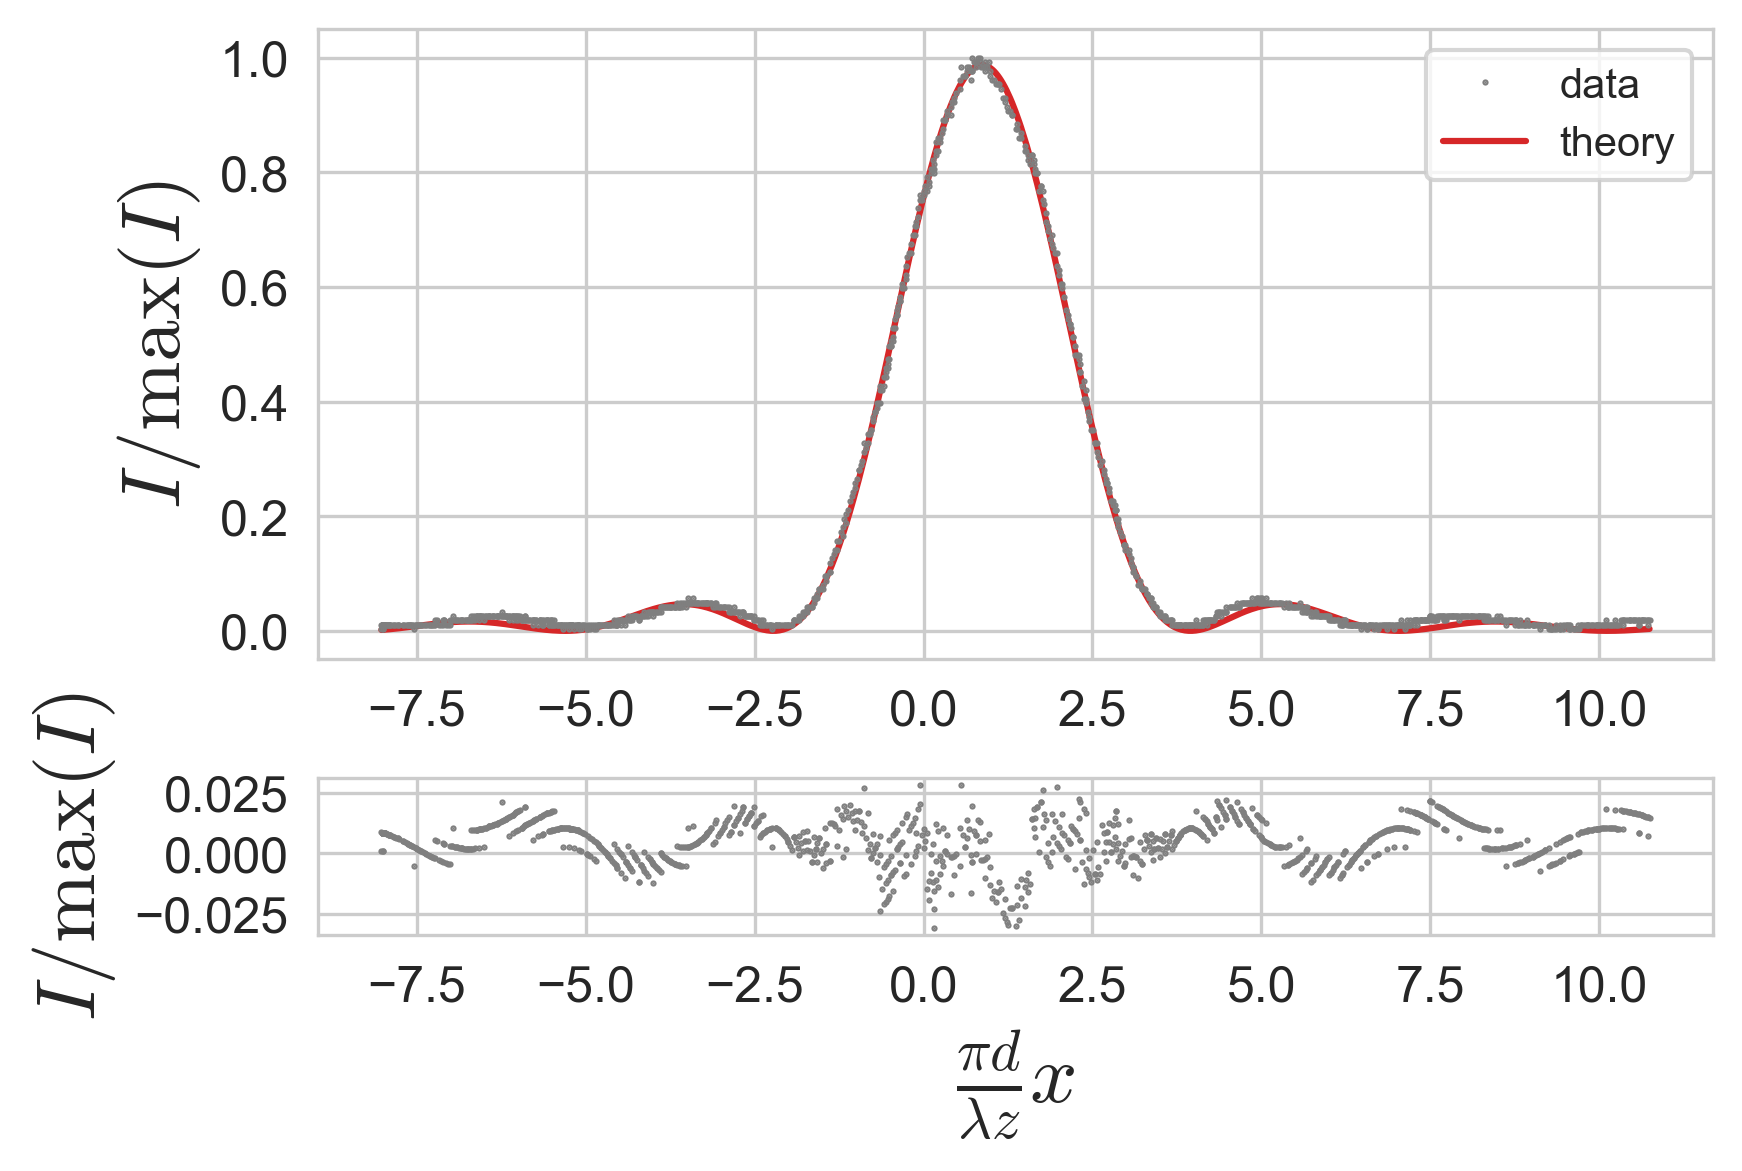
\includegraphics[width=0.9\columnwidth]{figures/single slit interference with 0.04mm width.png}
    \caption{$\lambda$ is the laser wave length $d$ is the width of the slit and $z$ is the distance from the screen}
    \label{fig:single slit interference with 0.04mm width}
\end{figure}
\begin{figure}[H]
	\centering
	\begin{subfigure}{0.5\columnwidth}
		\centering
		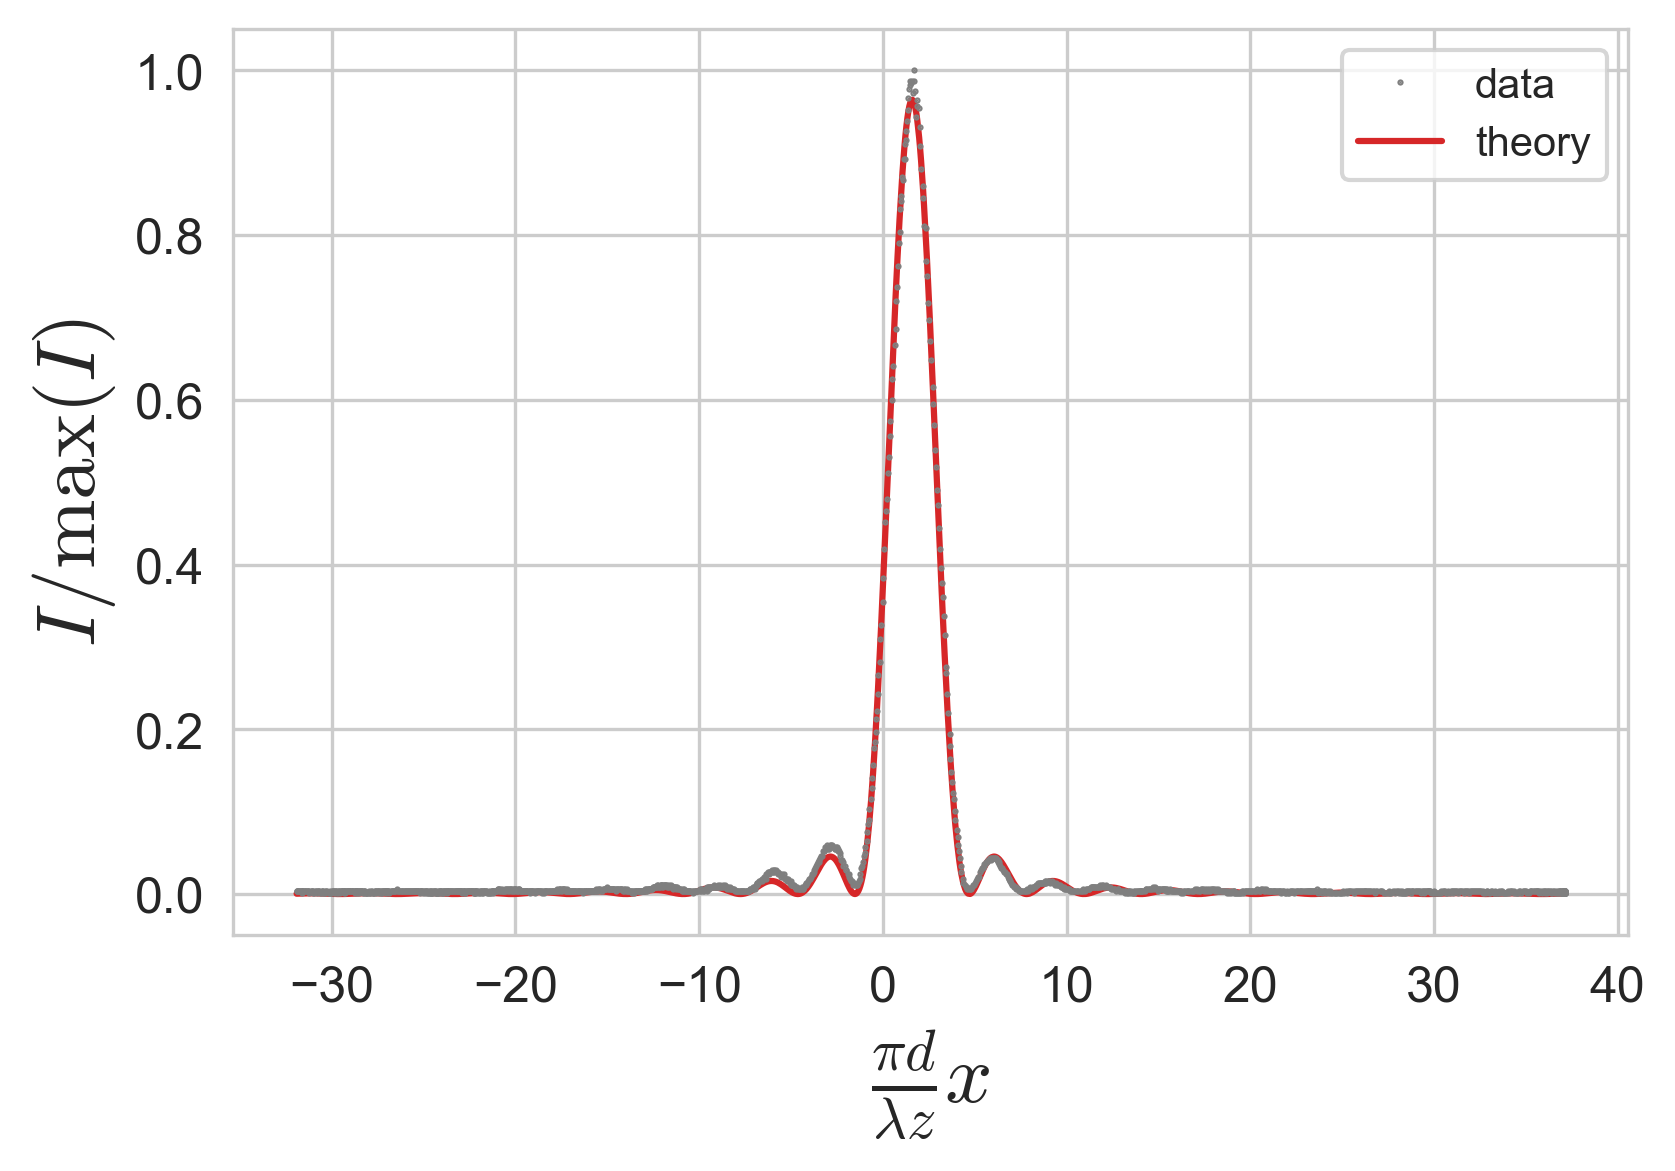
\includegraphics[width=\columnwidth]{figures/single slit interference 0.08mm.png} % first figure itself
		\caption{first figure}
        \label{fig:single slit interference 0.08mm}
	\end{subfigure}\hfill
    \begin{subfigure}{0.5\columnwidth}
        \centering
        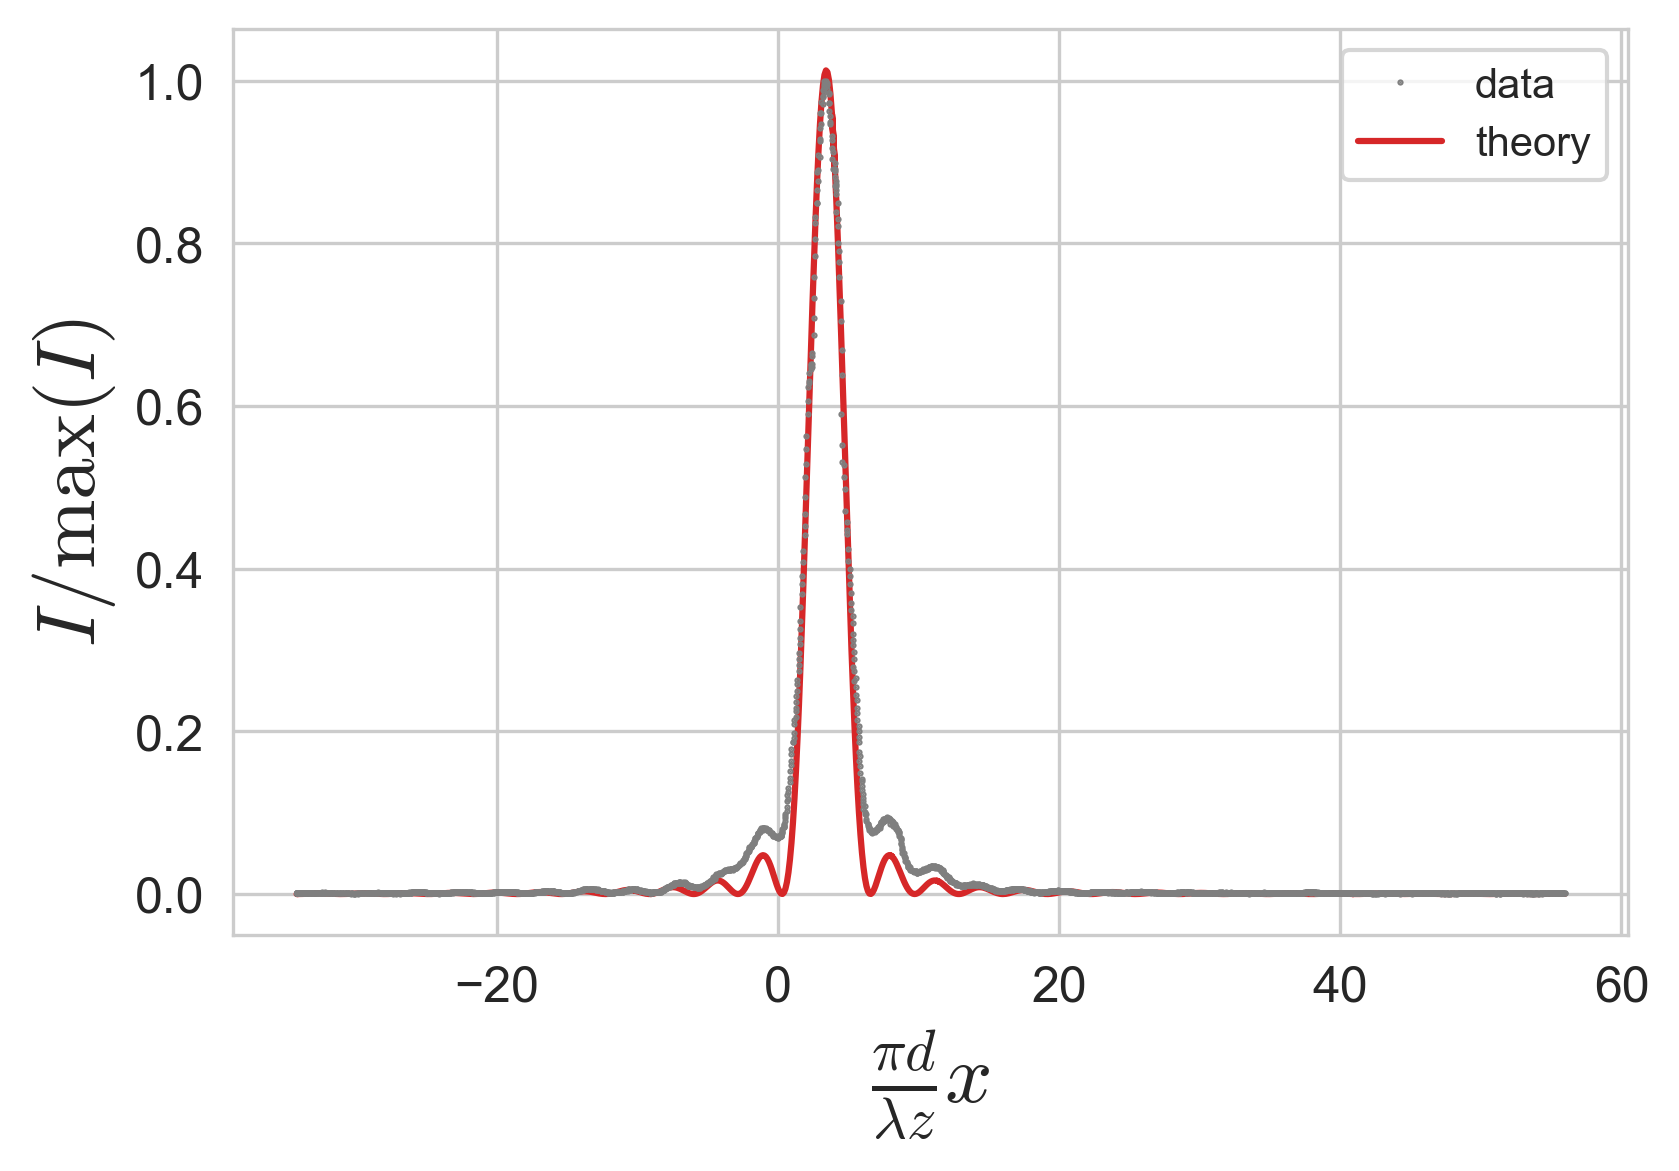
\includegraphics[width=\columnwidth]{figures/single slit interference 0.16mm.png} % second figure itself
        \caption{second figure}
        \label{fig:single slit interference 0.16mm}
    \end{subfigure}
    \label{fig:single slit examples}
\end{figure}

\begin{figure}[H]
    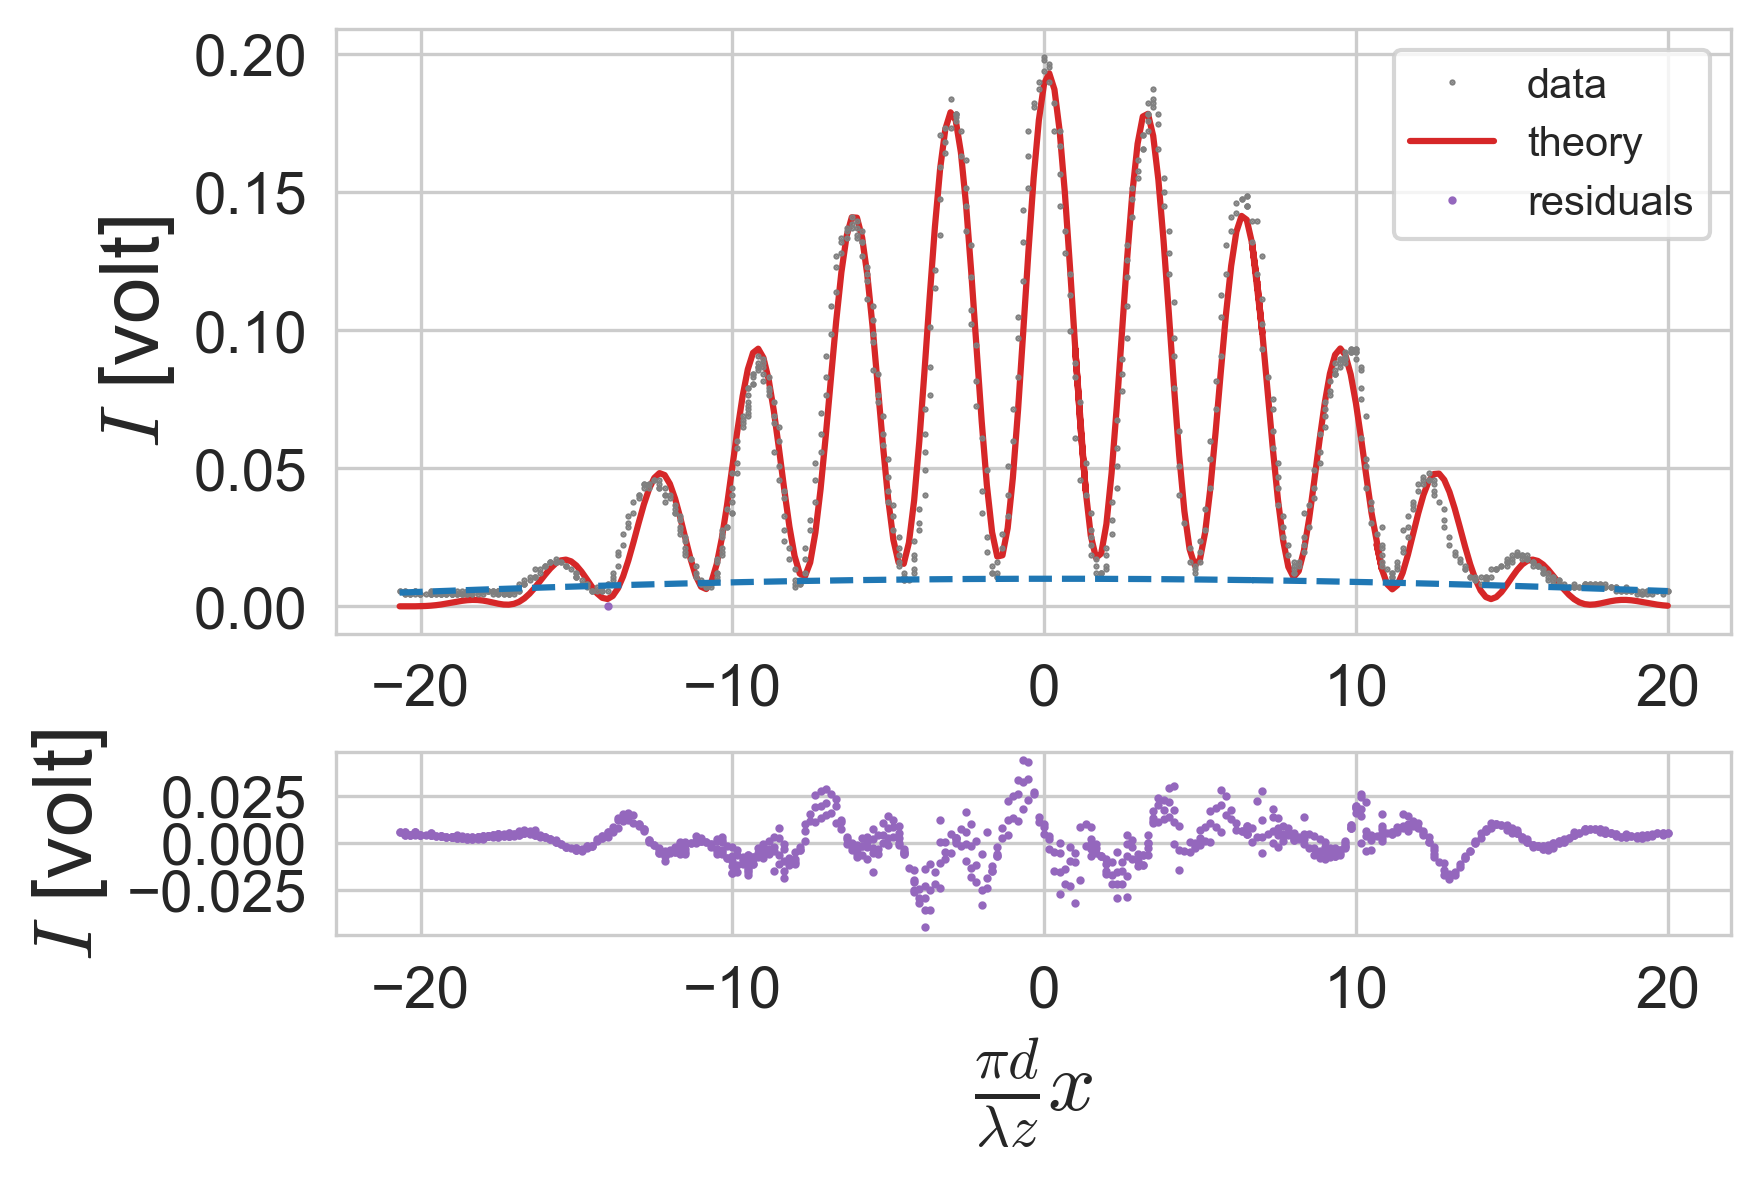
\includegraphics[width=0.9\columnwidth]{figures/0.04w0.25s memory.png}
    \caption{The secondary effects caused by measuring method are demonstrated here by the blue dashed line, we never see 0 intensity contrary to theory, and the visible offset in the fit relative to measurements. $(\sigma\sim0.01)$)}
    \label{fig:0.04w0.25s_memory}
\end{figure}
Two more evidence that the difference between model and measurement can be explained be our measuring tools is shown in Figure {\ref{fig:0.04w0.25s_memory}}.
The first being the fact that although we expect the intensity to approximately equal zero at some point along the x-axis, the local minima seem to increase in value closer to $x=0$.
This can be explained by the "iris effect" and the sensor's mechanism, that assign the sum of intensities at some neighborhood of a certain point to that point, specifically for the iris that neighborhood was estimated to be its' width.
The second effect we see is an offset between theory and experiment that is, especially around the tails, one-sided.
That tendency towards a certain side is duo to the fact that we scanned in a certain direction and the photoelectric sensor's measurement at a certain point is affected by measurements made a short time before that.
When taking into account the iris effect we saw an improvement in the fit.
According to the theory we used, the intensity for double slit patterns can be approximated as:\\
\[$I(x)=\frac{kd^2\cos^2\left(\frac{kLx}{2z}\right)sinc^2\left(\frac{dkx}{2z}\right)}{z\pi}$\]\\
As seen in Figure 6, when increasing the width of each slit we see that the $sinc$ function is narrower, and for greater spaces between slits we see the increase in the $cos$ function's frequency as expected.
What's not predicted by our theory is the decrease in maximum amplitude which shouldn't change when altering the spacing,
that can be explained by the fact we centered the maximum amplitude of the laser between slits for symmetry thus creating a decrease in amplitude of the incoming plane wave.
\begin{figure}[H]
    \centering
    \begin{subfigure}{0.5\columnwidth}
        \centering
        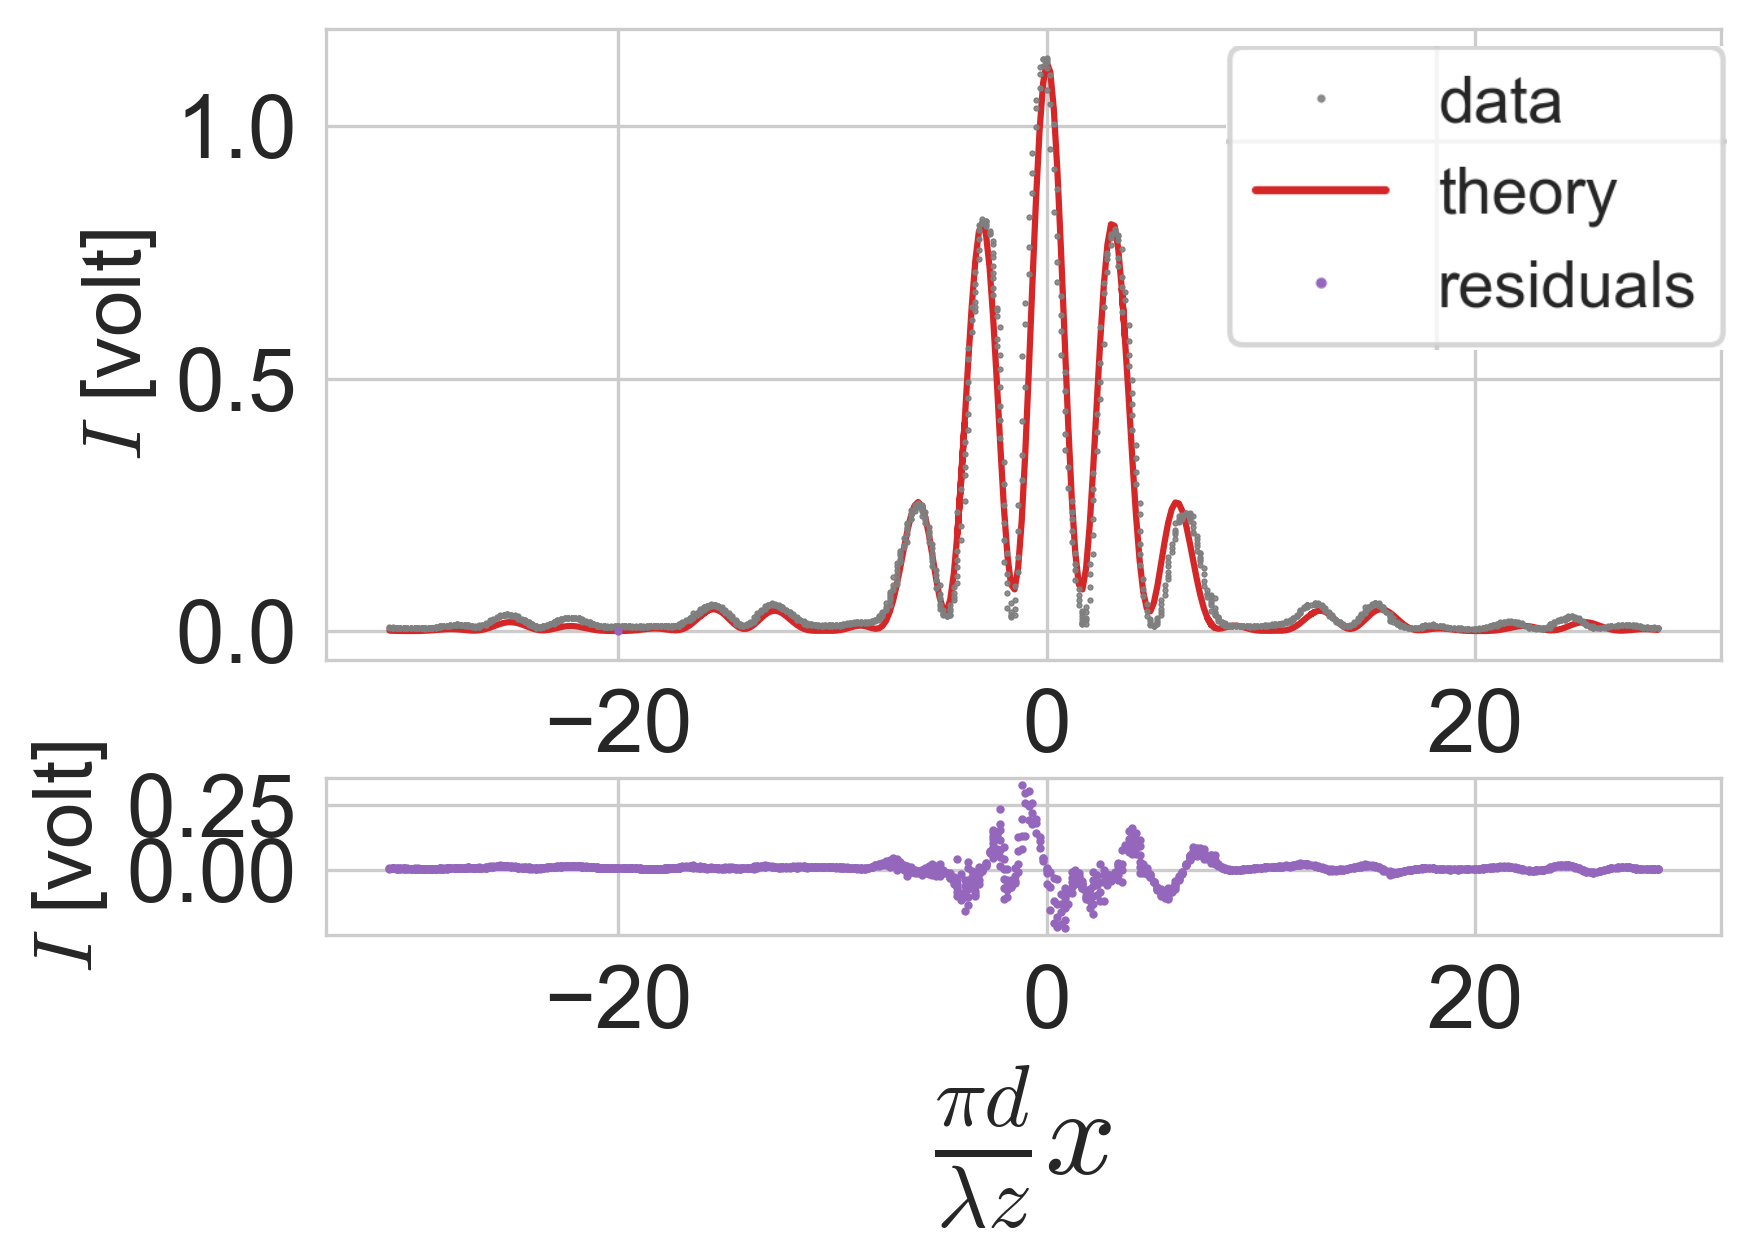
\includegraphics[width=\columnwidth]{figures/0.08w0.25s.png} % first figure itself
        \caption{\\$L=0.25[mm],d=0.08[mm]$}
        \label{fig:double slit interference 0.08w0.25s}
    \end{subfigure}\hfill
    \begin{subfigure}{0.5\columnwidth}
        \centering
        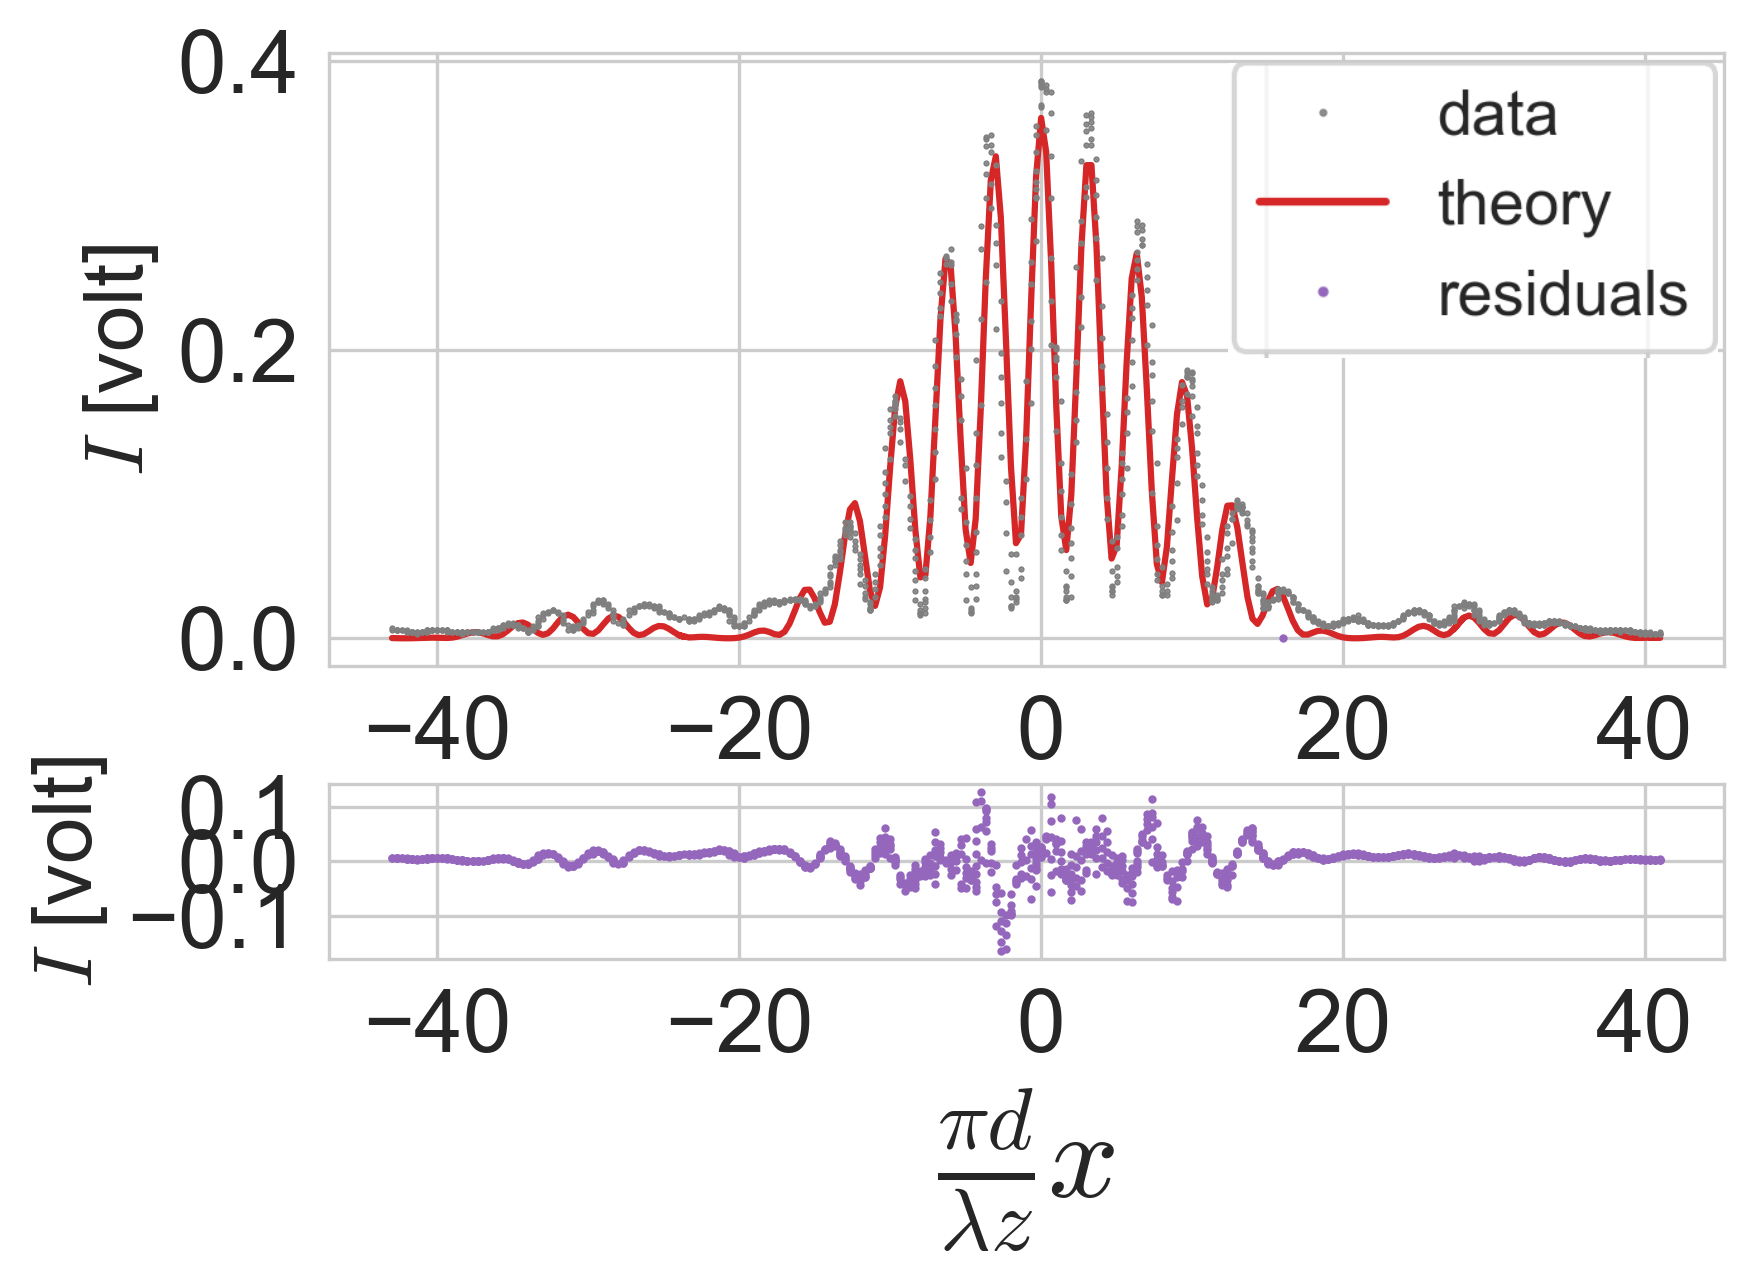
\includegraphics[width=\columnwidth]{figures/0.08w0.5s.png} % second figure itself
        \caption{\\$L=0.5[mm],d=0.08[mm]$}
        \label{fig:double slit interference 0.080.5s}
    \end{subfigure}
    \caption{Diffraction patterns for different slit patterns, for wider slits we get a narrow envelope of main peaks and for greater spacing we see denser peaks.}
    \label{other doubles}
\end{figure}
\begin{figure}[H]
    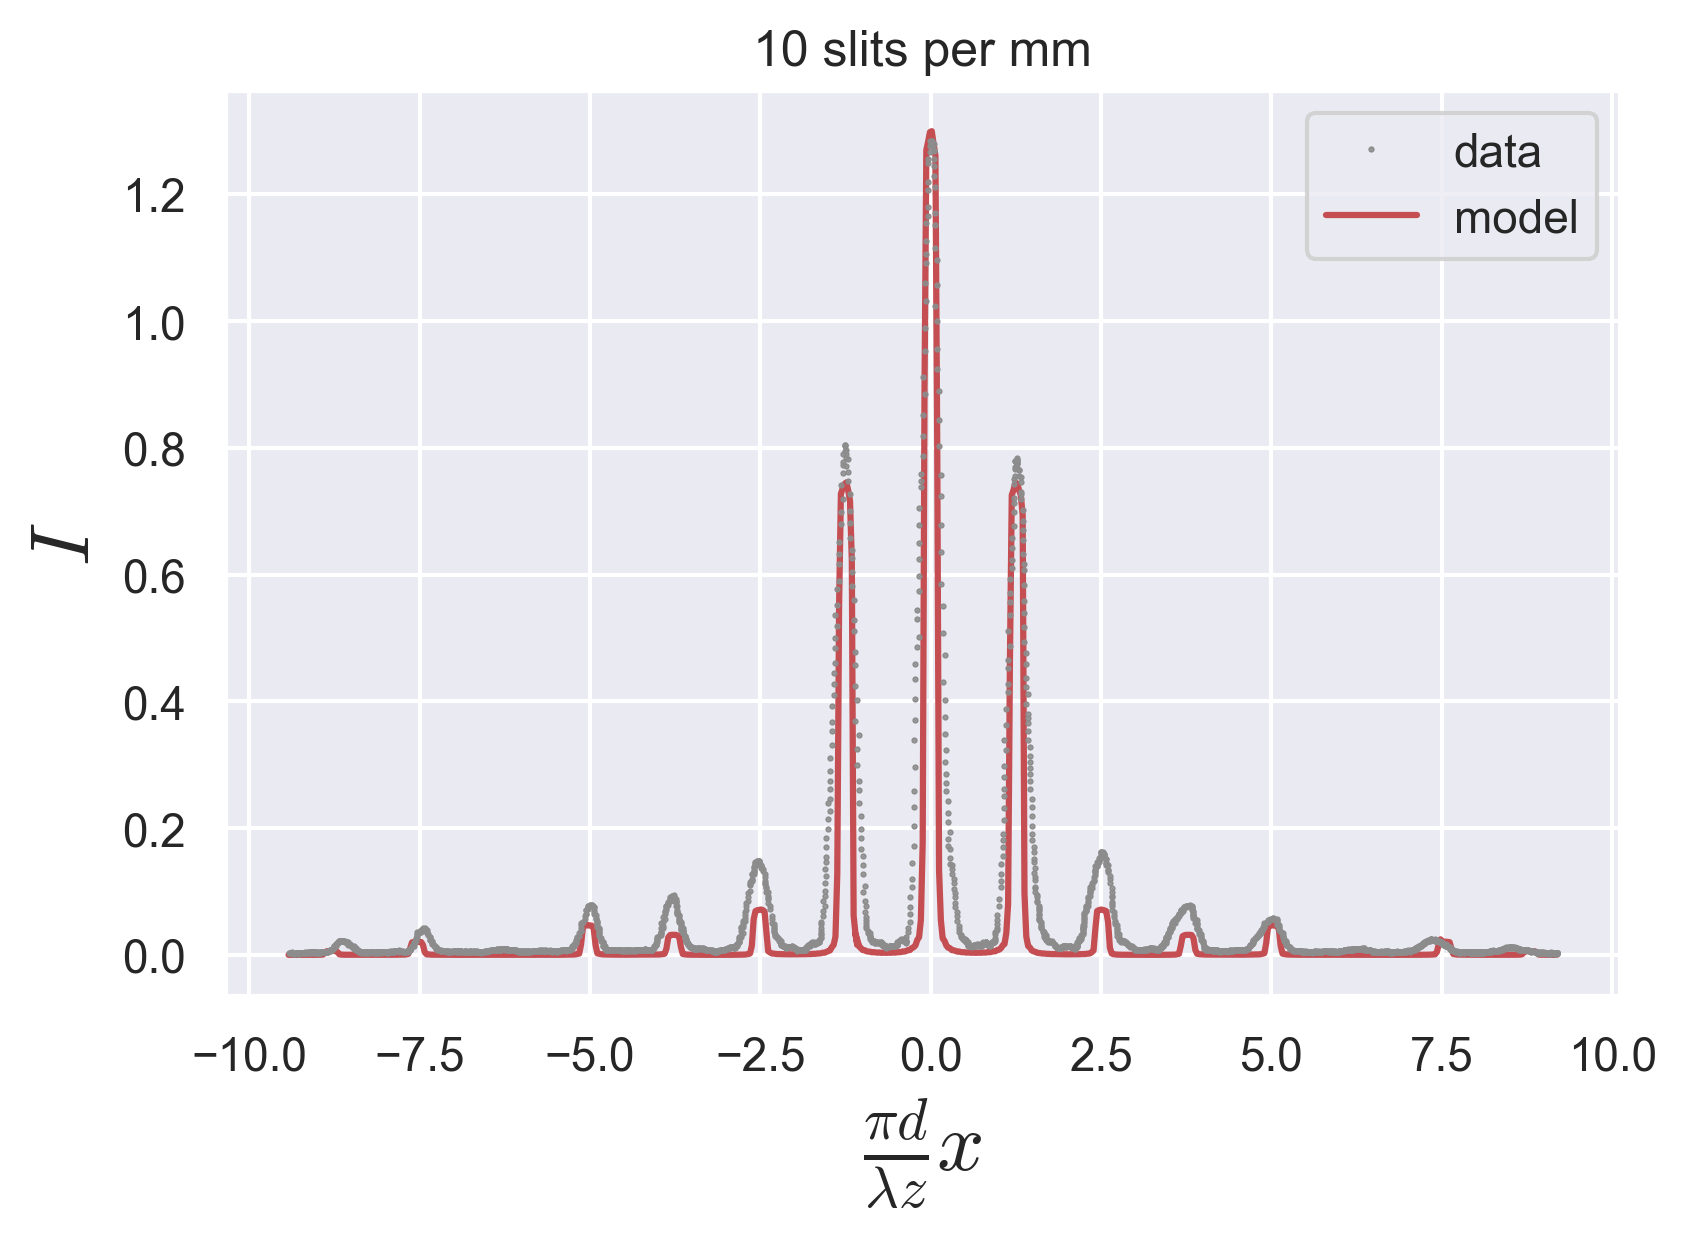
\includegraphics[width=0.9\columnwidth]{figures/10 slits per mm.png}
    \caption{}
    \label{fig:10 slits per mm}
\end{figure}
\newpage
In the case of the periodic diffraction grating "10 lines per mm" the secondary effects are more pronounced especially
the photoelectric sensor's "memory" (The photoelectric sensor has a relaxation period in which to voltage diminishes
therefore after exposure instead of an immediate cut off a slope can be seen as the voltage is recorded with the relation
to the angle which continues to change during said period giving us higher peaks and wider slopes near those peaks)\\
\\
Finally To justify the title of the paper we should look at the interference pattern of the helix (Which bears some resemblance the shape off DNA)
according to equation \eqref{eq:farfield} and the specified approximations the interference pattern can be calculated using
the 2 dimensional fourier transform of the shape of the slit, Taking the inverse fourier transform of the pattern should result
In the square of the shape of the slit (since when calculating the intensity the square of $U$ was taken)
as can be shown by \ref{fig:expansion inverse fourie transform}
\begin{figure}[H]
    \centering
    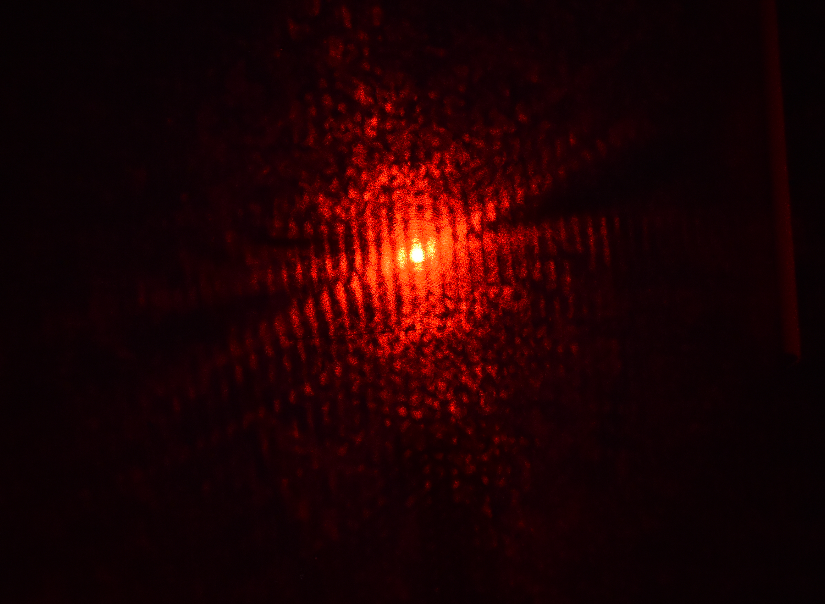
\includegraphics[width=0.9\columnwidth]{figures/expantion meshured interferemce.png}
    \caption{interference pattern measured as a result of diffraction with a helix}
    \label{fig:expansion measured interference pattern}
\end{figure}
\begin{figure}[H]
    \centering
    \begin{subfigure}{0.48\columnwidth}
        \centering
        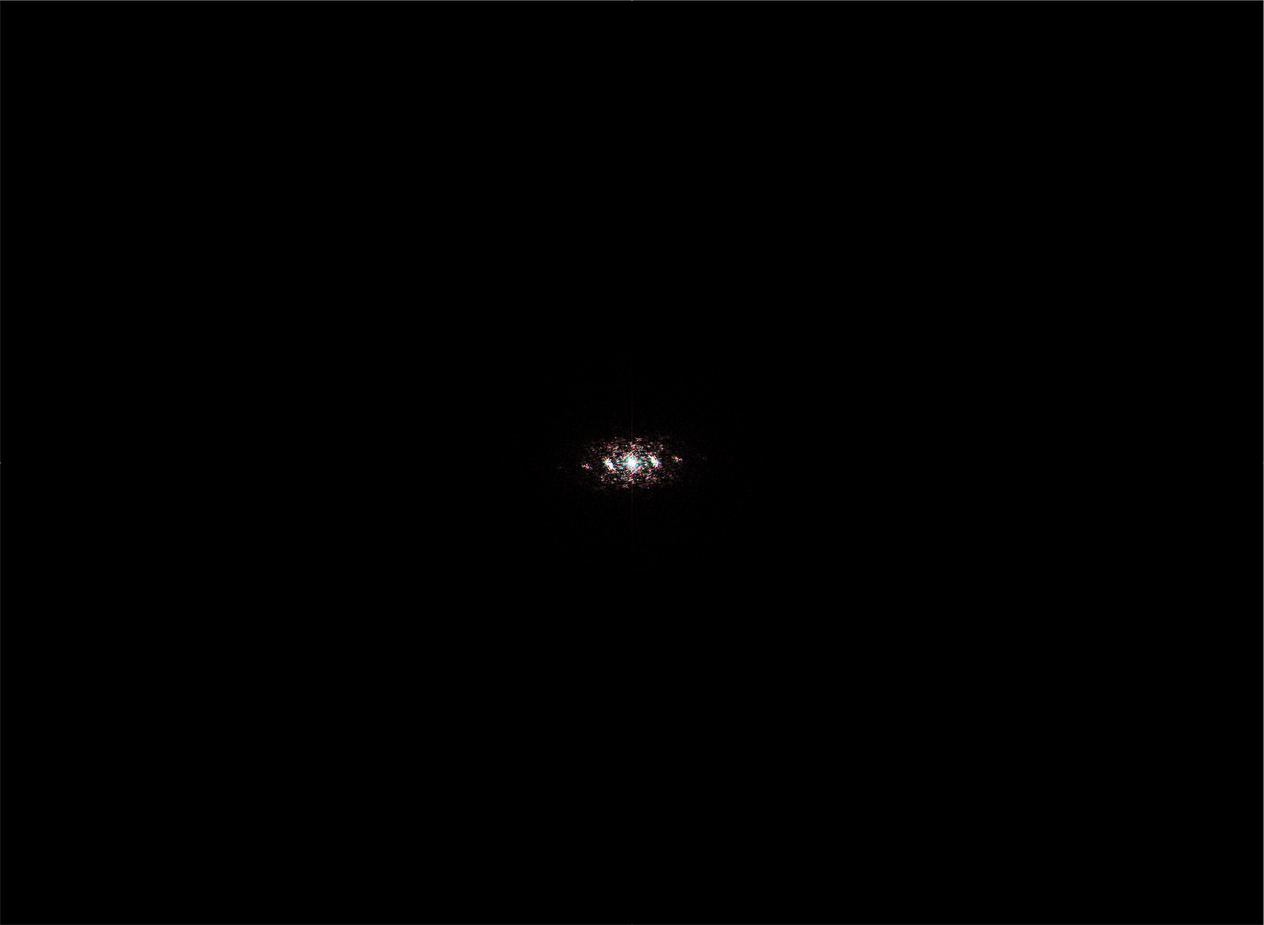
\includegraphics[width=0.9\columnwidth]{figures/expantion fourie transform.png}
        \caption{inverse discrete fourie transform calculated from the interference pattern at of the helix }
        \label{fig:expansion inverse fourie transform measured}
    \end{subfigure}\hfill
    \begin{subfigure}{0.48\columnwidth}
        \centering
        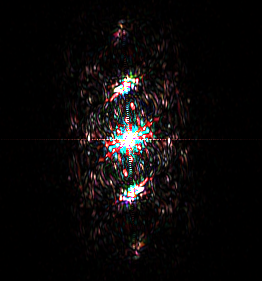
\includegraphics[width=\columnwidth]{figures/expantion fourie transform magnified.png} % second figure itself
        \caption{magnification of\ref{fig:expansion inverse fourie transform measured}}
        \label{fig:expansion fourie transform magnified}
    \end{subfigure}

    \label{fig:expansion theory measurements}
\end{figure}

As can be seen in \ref{fig:expansion fourie transform magnified} The result shows similarity to the calculation done in \ref{fig:expansion theory measurements}
in shape as in the orientation of the spring to the orientation of the "X"